\documentclass[tikz,border=8pt]{standalone}
% Shared look for every TikZ diagram. Load with % Shared look for every TikZ diagram. Load with % Shared look for every TikZ diagram. Load with \input{../../tools/tikz-style.tex}
\usepackage[T1]{fontenc}
\usepackage{lmodern}
\renewcommand{\sfdefault}{lmr}  % diagrams use the same serif as the text
\usetikzlibrary{arrows.meta, positioning, shapes.geometric, calc, fit, backgrounds}
\definecolor{cblue}{HTML}{4C78A8}
\definecolor{corange}{HTML}{F58518}
\definecolor{cgreen}{HTML}{54A24B}
\definecolor{cred}{HTML}{E45756}
\definecolor{cpurple}{HTML}{B279A2}
\definecolor{cgrey}{HTML}{6B6B6B}
\tikzset{
  every picture/.style={font=\sffamily, line width=1.2pt},
  box/.style={draw=#1, fill=#1!12, rounded corners=4pt, align=center, inner sep=7pt, minimum height=1.1cm},
  box/.default=cgrey,
  arrow/.style={-{Stealth[length=3mm]}, draw=cgrey, line width=1.4pt},
  title/.style={font=\sffamily\bfseries\Large},
  note/.style={font=\sffamily\small, text=cgrey, align=center},
}
\AtBeginDocument{\hyphenpenalty=10000 \exhyphenpenalty=10000}

\usepackage[T1]{fontenc}
\usepackage{lmodern}
\renewcommand{\sfdefault}{lmr}  % diagrams use the same serif as the text
\usetikzlibrary{arrows.meta, positioning, shapes.geometric, calc, fit, backgrounds}
\definecolor{cblue}{HTML}{4C78A8}
\definecolor{corange}{HTML}{F58518}
\definecolor{cgreen}{HTML}{54A24B}
\definecolor{cred}{HTML}{E45756}
\definecolor{cpurple}{HTML}{B279A2}
\definecolor{cgrey}{HTML}{6B6B6B}
\tikzset{
  every picture/.style={font=\sffamily, line width=1.2pt},
  box/.style={draw=#1, fill=#1!12, rounded corners=4pt, align=center, inner sep=7pt, minimum height=1.1cm},
  box/.default=cgrey,
  arrow/.style={-{Stealth[length=3mm]}, draw=cgrey, line width=1.4pt},
  title/.style={font=\sffamily\bfseries\Large},
  note/.style={font=\sffamily\small, text=cgrey, align=center},
}
\AtBeginDocument{\hyphenpenalty=10000 \exhyphenpenalty=10000}

\usepackage[T1]{fontenc}
\usepackage{lmodern}
\renewcommand{\sfdefault}{lmr}  % diagrams use the same serif as the text
\usetikzlibrary{arrows.meta, positioning, shapes.geometric, calc, fit, backgrounds}
\definecolor{cblue}{HTML}{4C78A8}
\definecolor{corange}{HTML}{F58518}
\definecolor{cgreen}{HTML}{54A24B}
\definecolor{cred}{HTML}{E45756}
\definecolor{cpurple}{HTML}{B279A2}
\definecolor{cgrey}{HTML}{6B6B6B}
\tikzset{
  every picture/.style={font=\sffamily, line width=1.2pt},
  box/.style={draw=#1, fill=#1!12, rounded corners=4pt, align=center, inner sep=7pt, minimum height=1.1cm},
  box/.default=cgrey,
  arrow/.style={-{Stealth[length=3mm]}, draw=cgrey, line width=1.4pt},
  title/.style={font=\sffamily\bfseries\Large},
  note/.style={font=\sffamily\small, text=cgrey, align=center},
}
\AtBeginDocument{\hyphenpenalty=10000 \exhyphenpenalty=10000}

% Section 3: alpha = a + b says how far out (the dashed lines); l1_ratio r = b / (a + b) says which direction.
% The four rows of the Note's table, all with alpha = 1, sit at (a, b) = (1 - r, r).
\begin{document}
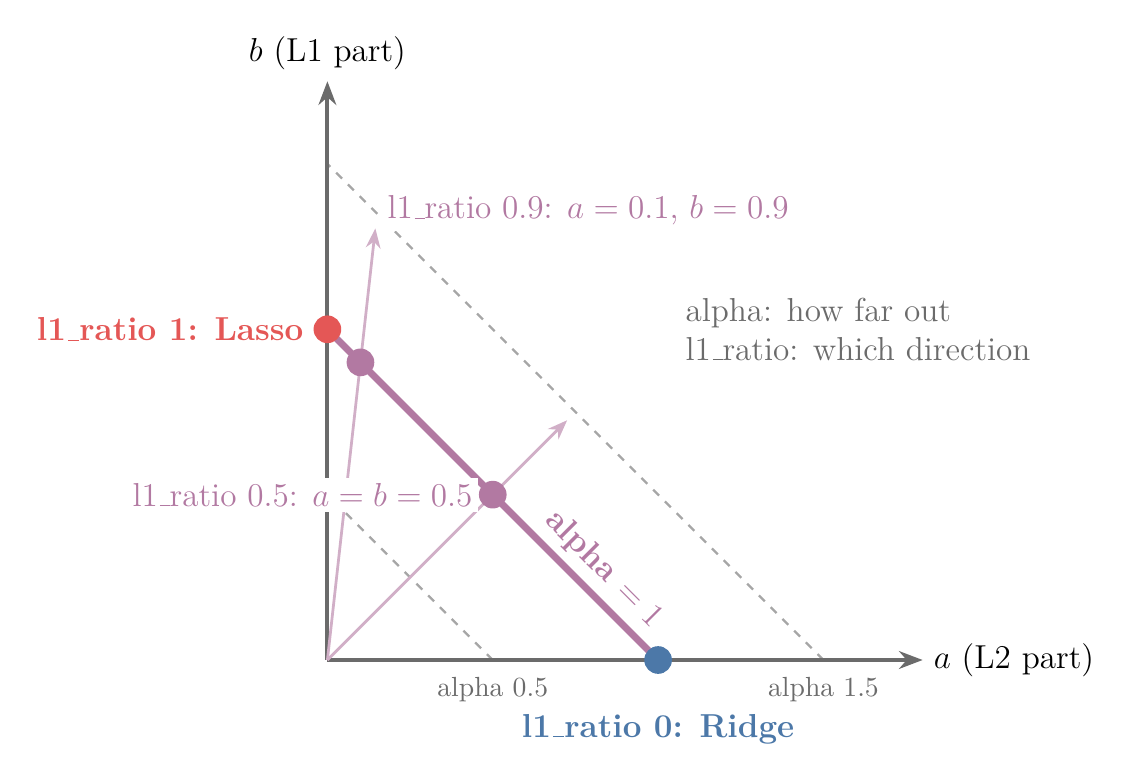
\begin{tikzpicture}[x=4.2cm, y=4.2cm]
  \foreach \t in {0.5,1.5} \draw[cgrey!60, dashed, line width=0.8pt] (\t,0) -- (0,\t);
  \node[note, font=\sffamily\normalsize, below] at (0.5,-0.02) {alpha 0.5};
  \node[note, font=\sffamily\normalsize, below] at (1.5,-0.02) {alpha 1.5};
  \draw[arrow] (0,0) -- (1.8,0) node[right, font=\sffamily\large] {$a$ (L2 part)};
  \draw[arrow] (0,0) -- (0,1.75) node[above, font=\sffamily\large] {$b$ (L1 part)};
  \draw[cpurple, line width=2.5pt] (1,0) -- (0,1);
  \node[font=\sffamily\bfseries\large, text=cpurple, rotate=-45, above] at (0.78,0.22) {alpha $= 1$};
  \foreach \r in {0.5,0.9} \draw[cpurple!60, line width=1pt, -{Stealth[length=2.5mm]}] (0,0) -- ({1.45*(1-\r)},{1.45*\r});
  \foreach \r/\c in {0/cblue, 0.5/cpurple, 0.9/cpurple, 1/cred} \fill[\c] ({1-\r},\r) circle (5pt);
  \node[font=\sffamily\bfseries\large, text=cblue, below] at (1,-0.13) {l1\_ratio 0: Ridge};
  \node[font=\sffamily\bfseries\large, text=cred, left] at (-0.04,1) {l1\_ratio 1: Lasso};
  \node[font=\sffamily\large, text=cpurple, left, fill=white, inner sep=2pt] at (0.46,0.5) {l1\_ratio 0.5: $a = b = 0.5$};
  \node[font=\sffamily\large, text=cpurple, right, fill=white, inner sep=2pt] at (0.16,1.36) {l1\_ratio 0.9: $a = 0.1$, $b = 0.9$};
  \node[note, font=\sffamily\large, align=left, anchor=west] at (1.05,1.0) {alpha: how far out\\l1\_ratio: which direction};
\end{tikzpicture}
\end{document}
